\chapter{Requirements}
\section{Functional requirements}


FR1 - Expert Interface\\
A crisis management expert should be able to set up a game template for teams to use. This interface should be able to configure as many variables in the game as possible(game rules), and be able to create maps, change the number of players, where they start, what events can occur and when, and create information cards.\\
\\
FR2 - Game Manager\\
An expert should be able to enter an existing game as a Game Manager. The GM should be able to trigger events and modify the game objects on the fly to make the game more dynamic, as well as comment on player actions. The GM should be able to monitor activity on the server, existing sessions and online players.\\
\\
FR3 - Player Profiles\\
Each player should have a profile that records the players performance in played games. This includes tracking wins and losses, listing game replays and other metrics that are relevant.\\
\\
FR4 - Replay\\
An expert should be able to view finished games as a re-play, to evaluate player performance. These replays should be stored in the database, to be viewed at any time.\\
\\
FR5 - Game functionality\\
In addition to adapting the functionality of the board game version to an electronic platform, as specified in appendix ~\ref{appendix:B}, the number of people in a zone should affect how panic spreads between zones, and inside them. \\
\\
FR6 - Physical interaction\\
Preferably, the game should be able to respond to commands sent by interaction devices such as Arduino or Sifteo cubes. They could be used to represent zones, players or be used as controllers for movement.\\
\\


\subsection{Use cases}
The use cases are mainly based on the functional requirements of the game and are a graphical representation of the users’ interactions with the board game. They document all the different ways in which the user can interact with the game. 
\\
A detailed set of use case diagrams and textual use cases are provided below.\\


\begin{figure}[H]
  \centering
    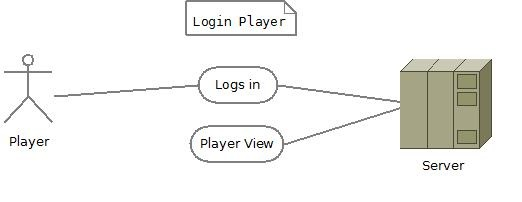
\includegraphics[width=1.0\textwidth]{img/loginplayer.jpg}
  \caption{Use case: Login player} 
  \label{fig:loginplayer}
\end{figure}


% START USE-CASE TABLES
\begin{table}[H]
\begin{tabular}{|l|p{14cm}|} \hline
	\textbf{ID} & \textbf{01}\\ \hline
	Corresponding FR & FR3\\ \hline
	Name & Login Player\\ \hline
	Goal & To be connected to the server\\ \hline
	Actors & Player, server\\ \hline
	Start requirements & None\\ \hline
	End requirements & - The player gets logged in.\\
					 & - The game is displayed.\\ \hline
	Case & - The player clicks on the option for player, in the middle of the HTML starpage\\
			& - The player gets prompted with the login form. \\
		 	& - The player gives login-info.\\
			& - The player clicks the login button to the rigth of the form.\\
			& - The player is now logged in.\\ 
			& - The player is moved to the player's page. \\ \hline
	Alternative Case & Wrong password\\ \hline
	Previous Use Case & None\\ \hline
	Spawned Use Case & 05\\ \hline
\end{tabular}
\caption{Use Case: Login player}
\label{fig:usecase01table}
\end{table}


\begin{figure}[H]
  \centering
    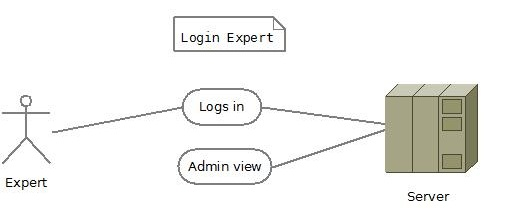
\includegraphics[width=1.0\textwidth]{img/loginexpert.jpg}
  \caption{Use case: Login expert} 
  \label{fig:loginexpert}
\end{figure}


\begin{table}[H]
\begin{tabular}{|l|p{14cm}|} \hline
	\textbf{ID} & \textbf{02}\\ \hline
	Corresponding FR & FR1\\ \hline
	Name & Login Expert\\ \hline
	Goal & To be connected to the server\\ \hline
	Actors & Expert, server\\ \hline
	Start requirements & None\\ \hline
	End requirements & - The expert gets logged in.\\
					 & - The expert view is displayed.\\ \hline
	Case & - The expert clicks on the option for expert in the middle of the HTML startpage\\
			& - The expert gets prompted with the login form. \\
		 	& - The expert gives login-info.\\
			& - The expert clicks the login button to the rigth of the form.\\
			& - The expert is now logged in.\\ 
			& - The expert is moved to the expert's page. \\ \hline
	Alternative Case & Wrong password\\ \hline
	Previous Use Case & None\\ \hline
	Spawned Use Case & 03, 09\\ \hline
\end{tabular}
\caption{Use Case: Login expert}
\label{fig:usecase02table}
\end{table}


\begin{figure}[H]
  \centering
    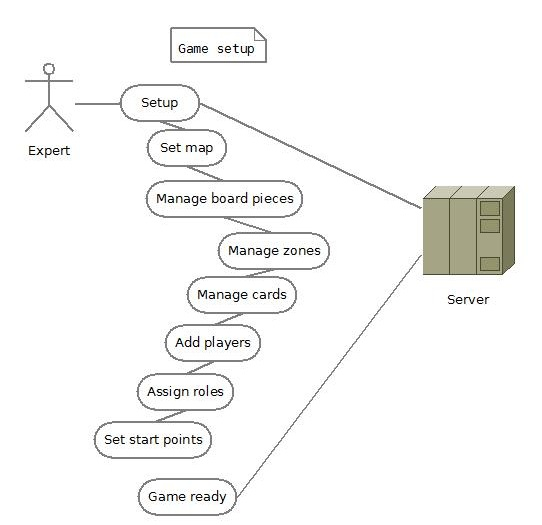
\includegraphics[width=1.0\textwidth]{img/gamesetup.jpg}
  \caption{Use case: Game setup} 
  \label{fig:gamesetup}
\end{figure}


\begin{table}[H]
\begin{tabular}{|l|p{14cm}|} \hline
	\textbf{ID} & \textbf{03}\\ \hline
	Corresponding FR & FR1\\ \hline
	Name & Game Setup\\ \hline
	Goal & To create a successful game session\\ \hline
	Actors & Expert, server\\ \hline
	Start requirements & The expert is logged in\\ \hline
	End requirements & The expert is able to create a game setup \\ 
						& The expert is able to save the game setup\\ \hline
	Case & - The expert creates the appropriate map for the game. By ploting nodes into the canvas
			and creates paths between them. To create a zone the expert selects a minimun of 3 paths and clicks for create zone.\\
			& - The expert adds the wanted board pieces by clicking on the corresponding buttons for the different game pieces, while in the wanted node. \\
			& - The expert selects what type of zone the selected zone should be, and does this for each zone.\\
			& - The expert set the number of people for each zone, by selecting a zone and using the initial people button at the top of the canvas.\\
			& - The expert sets the initial panic for each zone by selecting the zone and the corresponding button for initial panic, at the top of the canvas.\\
			& - The expert manages the cards, there is an initial set of cards for the game, but if the expert wants he can add more, or special cards at the top of the page, over the canvas for drawing the map.\\
			& - The expert adds the wanted number of players to the game, by selecting a node and by using the add player button.\\
			& - The expert can set a individual starting point to each player by selecting the wanted node and by using the button for add player at the top of the canvas.\\
			& - The expert assigns roles to each player, by selecting a player from the form over the canvas for creating the map. \\
			 \hline
	Alternative Case & None \\ \hline
	Previous Use Case & 02\\ \hline
	Spawned Use Case & 04, 05\\ \hline
\end{tabular}
\caption{Use Case: Game Setup}
\label{fig:usecase03table}
\end{table}


\begin{figure}[H]
  \centering
    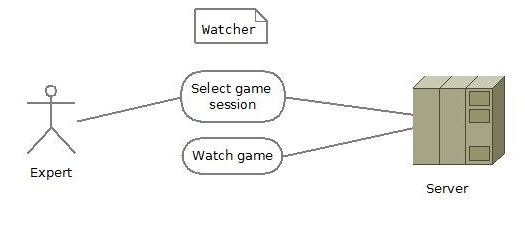
\includegraphics[width=1.0\textwidth]{img/watcher.jpg}
  \caption{Use case: Watcher} 
  \label{fig:watcher}
\end{figure}


\begin{table}[H]
\begin{tabular}{|l|p{14cm}|}
\hline
	\textbf{ID} & \textbf{04}\\ \hline
	Corresponding FR & FR2\\ \hline
	Name & Watcher\\ \hline
	Goal & To get a non player version of the game\\ \hline
	Actors & Expert, server\\ \hline
	Start requirements & The expert is logged in, a game is running \\ \hline
	End requirements & The expert is able to watch the wanted game\\ \hline
	Case & - From the monitor game option at the top of the expert page, the expert gets a list of games in session, the expert selects one of these to start monitoring the game.\\
		 & - The server provides a game window in which the expert is not participating as a player\\ \hline
	Alternative Case & None \\ \hline
	Previous Use Case & 02\\ \hline
	Spawned Use Case & None\\ \hline
\end{tabular}
\caption{Use Case: Watcher}
\label{fig:usecase04table}
\end{table}


\begin{figure}[H]
  \centering
    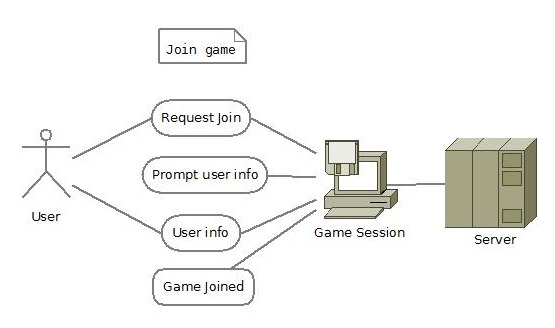
\includegraphics[width=1.0\textwidth]{img/joingame.jpg}
  \caption{Use case: Join game} 
  \label{fig:joingame}
\end{figure}


\begin{table}[H]
\begin{tabular}{|l|p{14cm}|}
\hline
	\textbf{ID} & \textbf{05}\\ \hline
	Corresponding FR & FR5\\ \hline
	Name & Join Game\\ \hline
	Goal & To successfully join a starting game\\ \hline
	Actors & User, game session, server \\ \hline
	Start requirements & A game has been created by the exper\\ \hline
	End requirements & A user is able to join the appropriate game\\ \hline
	Case & The user clicks on join options for the game in the middle of the page\\
			& - The game asks for user info in a popup form, the user enters the info. \\
			& - The user joins the game \\ \hline
	Alternative Case & The user gives incorrect info and is not added to the game \\ \hline
	Previous Use Case & 03 \\ \hline
	Spawned Use Case & 06, 07, 09\\ \hline
\end{tabular}
\caption{Use Case: Join Game}
\label{fig:usecase05table}
\end{table}


\begin{figure}[H]
  \centering
    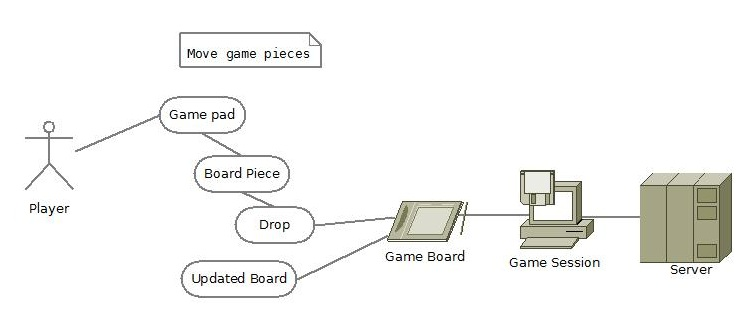
\includegraphics[width=1.0\textwidth]{img/movegamepieces.jpg}
  \caption{Use case: Move game pieces} 
  \label{fig:movepiece}
\end{figure}


\begin{table}[H]
\begin{tabular}{|l|p{14cm}|}
\hline
	\textbf{ID} & \textbf{06}\\ \hline
	Corresponding FR & FR5\\ \hline
	Name & Move game pieces \\ \hline
	Goal & To move a game piece to a wanted location \\ \hline
	Actors & Player, game board, game session, server \\ \hline
	Start requirements & The player has joined a game \\
				& The player in question has the turn \\ \hline
	End requirements & The player is able to move the selected piece to the wanted position. \\ \hline
	Case & - The player uses the mouse pad to select the wanted object. \\
		& - The player drags the object through the path to the wanted location. \\
		& - The game board is updated. \\ \hline
	Alternative Case & The player selects an immovable object \\
				& The player moves the object to an unobtainable location\\ \hline
	Previous Use Case & 06 \\ \hline
	Spawned Use Case & None\\ \hline
\end{tabular}
\caption{Use Case: Move game pieces}
\label{fig:usecase06table}
\end{table}


\begin{figure}[H]
  \centering
    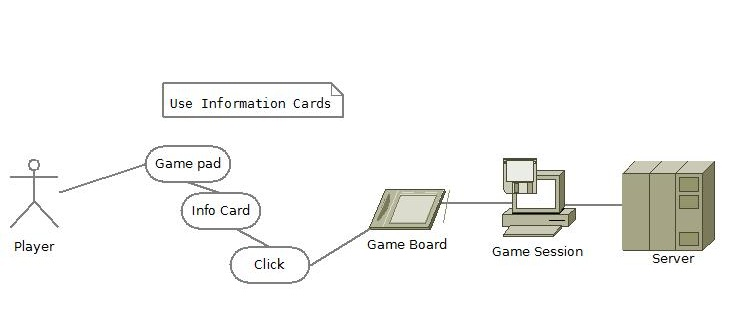
\includegraphics[width=1.0\textwidth]{img/useinfocards.jpg}
  \caption{Use case: Use information cards} 
  \label{fig:useinformationcards}
\end{figure}


\begin{table}[H]
\begin{tabular}{|l|p{14cm}|}
\hline
	\textbf{ID} & \textbf{07}\\ \hline
	Corresponding FR & FR5\\ \hline
	Name & Use information cards\\ \hline
	Goal & To use an information card to affect the board\\ \hline
	Actors & Player, Game Board, Game Session, Server\\ \hline
	Start requirements & The expert has created a game\\
				& The player is logged in\\
				& The player is part of a game\\
				& The player has an information card \\ \hline
	End requirements & The card effect is carried out on the board\\
				& The player does not have the used information card \\ \hline
	Case & The player clicks on the wanted information card under his player profile to the side of tha canvas.\\
		&- The information card effect is carried out on the board\\
		&- The player loses his information card \\ \hline
	Alternative Case & None \\ \hline
	Previous Use Case & 05\\ \hline
	Spawned Use Case & None\\ \hline
\end{tabular}
\caption{Use Case: Use information cards}
\label{fig:usecase07table}
\end{table}



\begin{figure}[H]
  \centering
    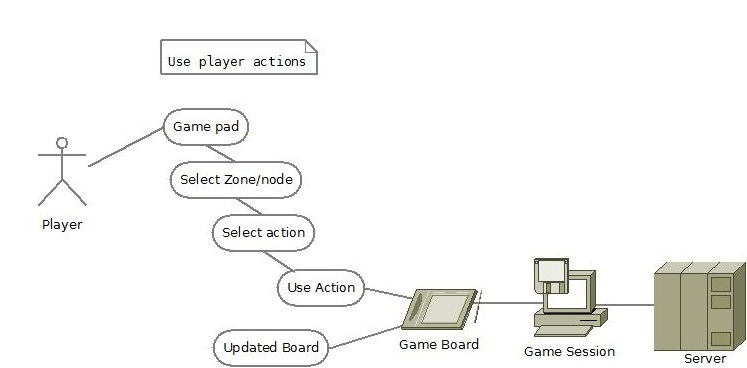
\includegraphics[width=1.0\textwidth]{img/useplayeractions.jpg}
  \caption{Use case: Use player actions} 
  \label{fig:useplayeractions}
\end{figure}


\begin{table}[H]
\begin{tabular}{|l|p{14cm}|}
\hline
	\textbf{ID} & \textbf{08}\\ \hline
	Corresponding FR & FR5\\ \hline
	Name & Use player action \\ \hline
	Goal & The player uses an action and the game board is updated\\ \hline
	Actors & Player, Game Board, Game Session, Server \\ \hline
	Start requirements & The user is logged in \\
				& The user is a player in the game\\
				& A game is in action\\ \hline
	End requirements & The player uses an action \\
				& The effect is updated on the board \\ \hline
	Case &- The player selects a adjacent node or a zone with the mouse pad.\\
		&- The player selects an action wich will appear at the top of the canvas after selecting a node or zone.\\
		&- The action is used on the target.\\
		&- The game board is updated.\\ \hline
	Alternative Case & None\\ \hline
	Previous Use Case & 05\\ \hline
	Spawned Use Case & None\\ \hline
\end{tabular}
\caption{Use Case: Use player actions}
\label{fig:usecase08table}
\end{table}



\begin{figure}[H]
  \centering
    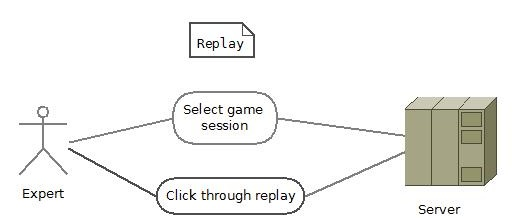
\includegraphics[width=1.0\textwidth]{img/replay.jpg}
  \caption{Use case: Replay} 
  \label{fig:replay}
\end{figure}


\begin{table}[H]
\begin{tabular}{|l|p{14cm}|}
\hline
	\textbf{ID} & \textbf{09}\\ \hline
	Corresponding FR & FR2\\ \hline
	Name & Watcher\\ \hline
	Goal & To watch a replay of a game session\\ \hline
	Actors & Expert, server\\ \hline
	Start requirements & The expert is logged in, a game session has been stored in the database. \\ \hline
	End requirements & The expert is able to click through the wanted game\\ \hline
	Case & - From the Replay option at the start of the page one can see all stored game sessions. The expert selects one game session, the replay is opened in the same window and is now ready. Using the buttons in the top right corner, the expert clicks forward or back in the replay.\\
	Alternative Case & None \\ \hline
	Previous Use Case & 02, 05\\ \hline
	Spawned Use Case & None\\ \hline
\end{tabular}
\caption{Use Case: Replay}
\label{fig:usecase09table}
\end{table}



% END USE-CASE TABLES



\section{Non functional requirements} 


All non functional requirements comply with the definitions as stated in the ISO 25010 standard (replacing ISO 9126). Only relevant requirements are mentioned in this report.

\subsection{Quality in use}

\emph{1: Efficiency}\\
Like regular board games, actions should not be difficult to execute. The players are working against the clock (the panic increase timer). Hence, when designing the user interface, one of the goals should be to minimize the number of clicks required.
\\\newline
\emph{2: Context Coverage}\\
The system should be flexible enough to accommodate individual experts’ preferences and needs in their simulations. By relying on the settings given by the expert through the expert interface form, the best possible flexibility can be ensured.

\subsection{Product quality}

\emph{1: Functional suitability}\\
Functional completeness should be achieved to include the core functionality 
of the board game, as well as the functionality specific to the electronic 
version, like the expert interface and panic- and people management. 
\\
Core functions must be without game-breaking bugs to ensure functional 
correctness.
\\\newline
\emph{2: Operability}\\
Usability is considered important, as the users should spend time playing the 
game and learn how to manage panic, rather than how to operate the game. 
\\
By exploiting recognisability from classic board games, a lot of interaction 
can be made intuitive, given that most people already know how to play board 
games. 
\\
Users of the game will most likely not be as proficient with computers as 
“gamers” in general. Therefore, it would be a good idea to make the game 
accessible without having to install any software other than an internet browser.
\\\newline
\emph{3: Transferability}\\
The client should be usable on as many platforms as possible (Mac, Windows, 
Linux, Mobile platforms), and in the best possible case be able to interact 
with devices such as Arduino. HTML5 with node.js was chosen for this reason, as 
it can run on nearly any device without the need for time consuming 
installation procedures, thereby increasing portability.


\subsection{Technical requirements}
These requirements have been copied from the “Don’t Panic” specifications 
provided by the customer.\\

Don’t Panic DPS has to meet to the following requirements:\\
- All interaction between the server and client SHOULD be performed using well 
documented protocols and standard protocols.\\
- The DPS Game rules SHOULD be platform independent. Consequently, high level 
languages such as Java, Processing, Python COULD be considered as good 
candidates.\\
- The overall architecture SHOULD be scalable to run multiple Game sessions in 
parallel without decreasing the quality of already running games sessions.\\
-Already existing frameworks for game development for such as Unity, Microsoft 
XNA Game Studio, or management tools such as RedMine COULD be used as platforms 
to help speeding up the development of the game. The choice should be driven by 
a framework comparison analysis considering both technical requirements and 
already existing skills/experience among group participants.






